The design of a robot manipulator can usually be divided into many parts.
It is divided into several structural elements that perform different functions and movements: the base, the body, the mechanical arm, the gripper. The latter, depending on the production requirements, is performed by: a gripper, when something needs to be moved, held or assembled; a welder - directly for welding products; a suction tool - to hold or move an object. From the base to the gripper, the robot is made up of links forming a kinematic chain. Two adjacent links form a kinematic pair. The distance from one link to another is called the link length. The distance from one degree of freedom to another is called the link distance. 


\begin{figure}[H]
	\centering
	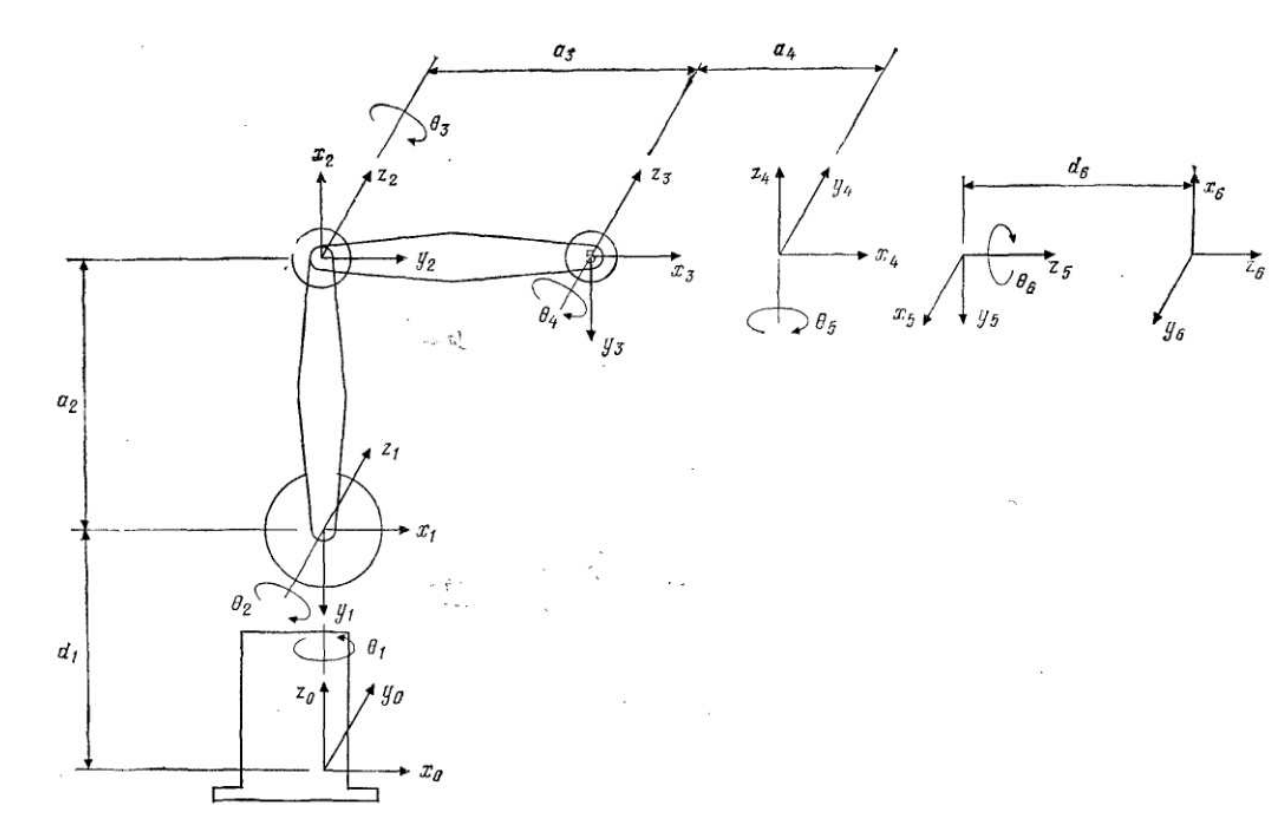
\includegraphics[width=0.7\textwidth]{Src/images/KinStr.png}
	\caption{Kinematic structure of robot manipulator}
    \label{kinematic1}
\end{figure}

Kinematic diagram of the manipulator robot presented in figure \ref*{kinematic1} 

\textbf{d5,d6} - Link distances 

\textbf{a2, a3, a4} - Link lengths 

\textbf{ \phi 1, \phi a2,\phi  a3,\phi a4, \phi 5 ,\phi 6} - Link angles